
\chapter{A method of continuation}\label{chap13}

\section{Principle of continuation}\label{chap13:sec1}

Give\pageoriginale $f \in \mathscr{H}_{\Lambda}(\Omega)$, first we shall find out a
method of continuation of $f$ to a point $Z$. Suppose that it is
possible to find a measure $d \mu = d \mu_Z$ with support in $\Omega$
such that $d \mu - \delta_z$ is orthogonal to $e^{\lambda z}$ for
every $\lambda \in \Lambda$, where $\delta_z$ is the Dirac measure at
$Z$. In other words, the following relation is given 
\begin{equation*}
  e^{\lambda z} = \int^{e^{\lambda z}} d \mu(z).\tag{1}\label{chap13:sec1:eq1}
\end{equation*}
We can try to replace $e^{\lambda z}$ by $f(z)$ in $(1)$, i.e. we can try to get 
\begin{equation*}
  f(Z) = \int f(z) d \mu (z). \tag{2}\label{chap13:sec1:eq2}
\end{equation*}

This is certainly possible when $Z \in \Lambda$, since $f \in
\mathscr{H}_{\Lambda}(\Omega)$. When $Z \notin \Omega$ this gives a
means of defining $f$ at $Z$. More precisely, if $f$ can be
approximated by $\sum a (\lambda) e^{\lambda z}$ in $\Omega$, then
formally we have the following relations 
\begin{align*}
 f(Z) & - \sum a (\lambda) e^{\lambda Z} = \int_K [ f(z) - \sum a
 (\lambda) e^{\lambda z}] d \mu_Z(z); \\ 
 |f(z) & - \sum a (\lambda) e^{\lambda z}| < \varepsilon \int | d \mu_z|
\end{align*}
Hence the majorization does not depend on $Z$ but on $d \mu_z$. If $Z$
belongs to a continuum $\mathscr{C}$ and if it is possible to
find a measure $d \mu_z$ with support in $K \subset \Omega, K$
independent of $Z$, such that $\int |d \mu_z| < B$ uniformly in $Z$,
then $f$ can be approximated on $\mathscr{C}$ by the same sums $\sum
a(\lambda)e^{\lambda z}$ as on $K$ and $\sup \limits_{Z \in
 \mathscr{C}} |f(Z)| \le \const \max \limits_{z \in K}|f (z)|$. To
find the measure $d \mu$ is exactly the same thing as to find its
Fourier transform. In other words, we seek an entire function $M(w) =
M_Z(w)$ of exponential type with conjugate diagram in $\Omega$ such
that $- M(w) + e^{wZ}$ vanishes for $w \in \Lambda$ 

Moreover,\pageoriginale we want $M (w)$ to be the type $M (w) = \dfrac{1}{ 2\pi i}
\int_C^{\varphi_Z^{(z)} e^{wz}{dZ}}$, $C$ being a curve in
$\Omega$ fixed for all $Z$, and $\varphi_Z(z)$ uniformly bounded on
$C$ when $Z$ belongs to a given continuum. According to formulae
(\ref{chap13:sec1:eq1}) 
and (\ref{chap13:sec1:eq2}) in lecture \ref{chap9}, this last
condition is satisfied whenever $M_{Z}(w)$ admits a uniform majorization 
\begin{equation}
 |M_Z (w)| < \frac{K}{1+r^2} e^{rk(\theta)} (w = r e^{i \theta})
 \tag{3}\label{chap13:sec1:eq3} 
\end{equation}
and $C$ is the frontier for the convex set defined by 
\begin{equation}
 X \cos \theta - y \sin \theta \leq k (\theta) \tag{4}\label{chap13:sec1:eq4}
\end{equation}

Then, (\ref{chap13:sec1:eq2}) can be written as 
\begin{equation}
 f (Z) = \frac{1}{2 \pi i } \int_C \varphi_Z (z) f (z) dz
 \tag{5}\label{chap13:sec1:eq5} 
\end{equation}

Let us remark that (\ref{chap13:sec1:eq3}) need not be required for every $\theta$; if
$C$ can be defined from (\ref{chap13:sec1:eq4}) with $ \theta \in S, S$ being a
given subset of [$0,2n$], it is sufficient to have
(\ref{chap13:sec1:eq3}) when $ \theta 
\varepsilon S$, and to assume that $M_Z(w)$ is of exponential type; in
particular, if $C$ is a convex polygon, $S$ can be taken as a
discrete set; in this case, we shall say \textit{``$S $ is
 associated with $C$''}. 

Thus the principle of continuation can be formulated as follows: Let $D
(w)$ be an entire function of exponential type, vanishing $\Lambda$,
with its conjugate diagram $J$ contained in $\Omega$. Let $C$ be a
convex polygon contained in $\Omega$, and containing $J$ in its
interior, and let $S$ be a set associated with $C$. Let $Z \in
G$, and suppose that, for each $Z$, there exists a meromorphic
function $A (w) = A_Z (w)$, with polar part $\sum\limits_{ \lambda
 \in \Lambda} \dfrac{e^{\lambda Z}} {D' (\lambda) (w-
 \lambda)}$ uniformly bounded when $\theta \in S$, and also
when $|w| = R_j \lim R_j = \infty$. Then $C$ and $M_Z(w) = D (w) A_Z
(w)$ satisfy the condition above. If we put 
\begin{equation}
 \varphi_ z(w) = \int\limits^{\infty{^{ i \alpha}}}_0 D (w) A_Z (w)
 e^{- wz} dw \tag{6}\label{chap13:sec1:eq6} 
\end{equation}
and\pageoriginale if $f \in \mathscr{H}_\Lambda (\Omega)$,
(\ref{chap13:sec1:eq5}) defines a
continuation of $f$ in $G$, in such a manner that $1^0)$ on $G$~ $f$
is a uniform limit of the same Dirichlet polynomials $\sum a
(\lambda) e^{\lambda z} (\lambda \in \Lambda)$ as on $C$ (in
particular, if $G$ is an open set, $f$ is analytic on $G$, if $G$ is
an open set and $G \cap \Omega \neq \phi$, (\ref{chap13:sec1:eq5}) provides an analytic
continuation of $f$ from $\Omega$ into $G$). 
\begin{equation*}
  2^0) \text{ on } G, |f (Z) |<
  K \sup\limits_{Z, \in C} |f (z)|, K \text{ independent of }
  Z. \tag{7}\label{chap13:sec1:eq7}  
\end{equation*}

Let us remark that, if $\Lambda$ is the sequence of the negative
integers, our principle of continuation gives the same result as the
Cauchy formula, translated after a change of variable $\zeta =
e^{-z}$. Thus, (\ref{chap13:sec1:eq5}) is a kind of generalization of the Cauchy
formula. 

\section{Application of the principle of continuation}\label{chap13:sec2}%Sec 2

We have a solution of the problem of continuation of we can construct
the function $D (w)$ and $A (w)$ satisfying the above principle. We
shall apply this principle directly in simple cases and with a little
modification in other cases, for example for $\mathscr{C}_\Lambda (K),
K \subset R$; then we shall obtain, for certain real sequence
$\Lambda$, the analytic continuation of $f \in
\mathscr{C}_\Lambda (K)$; this forms the main result in the thesis of
$L$. Schwartz (Schwartz $1$ (see lecture \ref{chap16})). In certain cases, we
shall take $A (w)$ having an integral representation of the form $A(w)=
\lim\limits_{ j \to \infty} \int_{C_j} \dfrac{e^{w'Z} dw'}{D (w')
 (w-w')}, C_j$ being certain closed curves (see lecture \ref{chap15}). 

We first apply this principle in the simplest way. We suppose
$\Lambda$ is a negative sequence,viz. every element of $\Lambda$ is a
negative number $\Lambda = \{ \lambda\}_{\lambda < 0}$. The required
$D(w)$ is provided by the canonical product $D (w) = C (w) = \prod
\limits_{ \lambda \in \Lambda} ( 1 - \frac{w^2}
  {\lambda^2})$. This begin achieved, to construct $A(w)$, we
  make some more assumptions on $\Lambda$ in such a way that the
  polar part of $A(w)$\pageoriginale is normally convergent outside the union
  of small circles $U_\lambda= \{ |w -\lambda| < \rho\}, A (w)$
  being uniformly majorized outside these small circles. 

\noindent I. Let $\Lambda$ possess a density $D$. 

 We have $D (w) = C(w)= \prod (1- \frac{w^2} {\lambda^2})$ and the
 conjugate diagram of $C(w)$ is the segment joining $i \pi D$ and $-i
 \pi D$. We take $\Omega$ to be a small domain containing this
 segment so that $f$ is analytic in $\Omega$. Suppose $A(w)$ is of
 the form 
 \begin{equation*}
   A (w) = \sum \frac{ e^{\lambda Z}} {C' (\lambda) (w -\lambda)}
   \tag{1}\label{chap13:sec2:eq1} 
 \end{equation*}

 In order that this series is normally convergent when $Z = X + iY$
 varies outside $U_\lambda= \{ \big|w-\lambda\big| < \zeta \}$, it is
 sufficient to have $ \exp (\lambda X - \log |C' (\lambda)|) < e
^{\lambda \varepsilon}$ or again the following relation 
 $$
 X > \delta + \varepsilon, \varepsilon > 0, \text{ where } \delta =
 \lim \sup \frac{ \log |C' (\lambda)|} {\lambda}. 
 $$

 \begin{defi*}
   When $\Lambda$ possesses a density $D, \delta = \lim \sup \frac{
     \log |C' (\lambda) |} {\lambda}$ is defined as the \textit {``
     index of condensation''} of $\Lambda$. 

 A sequence $\Lambda$ is called ``regular'' if $\lim \limits_{
  \lambda' \neq \lambda} \sup | \lambda' - \lambda| > 0$. If
 $\Lambda$ is a regular sequence it can be proved (V. Bernstein,
 note II) that $\delta = 0$. When $\delta = 0$. we have the 
 \end{defi*}

 \begin{theorem*}
 Let $\Lambda$ be a negative sequence with density $D$ and let $
 f \in \mathscr{H}_\Lambda (\Omega)$, $\Omega \supset [-i \pi D, i
  \pi D]$. When $\delta=0$, every function $f \in
 \mathscr{H}_\Lambda(\Omega)$ can be continued
 analytically in the right half plane $x \ge 0$ into a sum of
 convergent Dirichlet's series $\sum a (\lambda)e^{\lambda z}$ 
 \end{theorem*}

 As a consequence of this theorem we obtain a classical result on
 Dirichlet's series. Let $f (z) = \sum a(\lambda) e^{\lambda z}$ be
 a Dirichlet's series where $\Lambda$ is a sequence of positive
 number having $\infty$ as the sole limit point. If $f (z)$ is
 convergent for $Re Z = x_o $, it is also convergent for\pageoriginale $Re Z = x
 > x_o$. Thus one can define the abscissa of convergence, 
 $\sigma_a$, as an ordinate through $x =\sigma_a$ to the right of
 which $\sum a (\lambda ) e^{\lambda z}$ is convergent and to the
 left of which $\sum a (\lambda)e^{\lambda z}$ is not convergent 

 We have the following corollary:
 \begin{coro*}
 The Dirichlet's series $\sum a (\lambda) e^{\lambda z}$ with
 exponents extracted from a sequence having a density $D$ and
 index of condensation zero, admits at least one singularity on
 every segment of length $2 \pi D$ on its abscissa of
 convergence. If $D = 0$ and if $ \Lambda$ is a sequence of
 integers, the change of variables $\zeta = e^{-z}$ gives the Fabry
 theorem, viz., the circle of convergence is the natural boundary
 of a gap series. 
 \end{coro*}
 
\noindent 
\begin{minipage}[c]{7cm}
 \begin{proof of the corollary}
 Indeed if there is no singularity, $\Omega$ can be taken very
 narrow containing this segment and the Dirichlet's series is
 ultra-convergent in $\Omega$ (lecture 12, \ref{chap12:sec2}). Taking a segment
 of length $2 \pi D$ in $\Omega$ parallel to this segment and to
 the left of the abscissa of convergence $\sigma_f $ we see by
 the above theorem that the Dirichlet's series is convergent to the
 left of $\sigma_f$, which is impossible. 
 \end{proof of the corollary}

 Let $\sigma_k$ (``abscissa of holomorphy") be the infimum of the
 $\sigma$ such that $f (z) = \sum a (\lambda) e^{\lambda z}$ is
 analytically continuable for Rez $ > \sigma$. When $\delta \neq 0$
 and if $ \sigma_h$ and $\sigma_c$ are the abscissa of holomorphy
 and convergence of Dirichlet's series $\sum a (\lambda) e^{\lambda
 z},$ applying as above the result about ultra-convergence and the
 condition that it converges for $ x > \sigma_h + \delta +
 \varepsilon$ we obtain the following result of V. Bernstein. 
\end{minipage}
\begin{minipage}[c]{2.9cm}
\begin{figure}[H]
\centerline{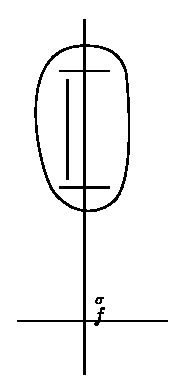
\includegraphics{vol15-figures/fig15-6.eps}}
\end{figure}
\end{minipage}
\medskip

 \begin{theorem*}
 $\sigma_c - \sigma_h \le \delta$,\pageoriginale and every segment of length $2
 \pi D$ on Re $z = \sigma_h$ contains at least one singularity. 
 \end{theorem*}

 Suppose now $f (z)$ is an entire function, $f (z) = \sum\limits_{
 \lambda \in \Lambda} a(\lambda) e^{- \lambda z}$. The
 inequality (\ref{chap13:sec1:eq7}) allows us to compare the order of magnitude of $f$
 in the whole plane and in the strip, when $x =Re z \to -
 \infty$. Let $\mathscr{Y}$ be a horizontal strip of width $2 \pi D
 + \varepsilon, M (x) = \sup\limits_{ Rez=x} |f (z)|$ 
\begin{figure}[H]
\centerline{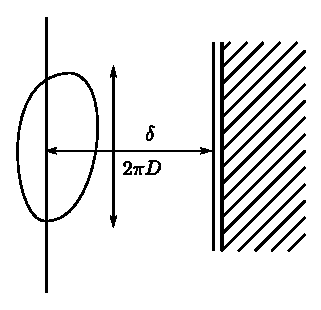
\includegraphics{vol15-figures/fig15-7.eps}}
\end{figure}

 $M_\mathscr{Y} (x) \sup\limits_{ Rez=x, z \in \mathscr{Y}}
 |f (z)|$. We have immediately 
 \begin{theorem*}
 $M (x) \le K M_\mathscr{Y} (x - \delta - \varepsilon ' ), K$
 depending only on $\Lambda, \varepsilon$ and $\varepsilon '
 (\varepsilon > 0, \varepsilon ' > 0 ~\text{ width of}~ \mathscr{Y} = 2
 \pi D + \varepsilon)$ 
 \end{theorem*}

 We obviously get the same result on supposing $\mathscr{Y}$ to be a
 curvilinear strip. 

\noindent II. Let the sequence $\Lambda$ possess a finite mean upper
density $\bar{D}^.$. 
 If $\Lambda$ is regular and $\big| \lambda' - \lambda \big| > h > 0$,
 it has been proved by S. Mandelbrojt that $\lim \sup \frac{ \log |C'
 (\lambda)|} {\lambda} = \delta < B$, where $B = B (\bar{D}^., h)$ is
 a constant depending on $\bar{D}^.$. and $h$ (Mandelbrojt 2, 3). 

\begin{figure}[H]
\centerline{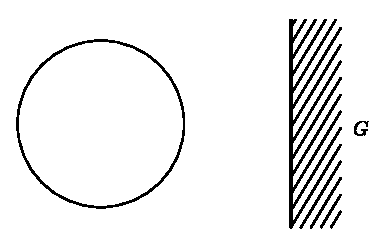
\includegraphics{vol15-figures/fig15-8.eps}}
\end{figure}

We know that the conjugate diagram of $C (w)$ is contained in a circle
of radius $\pi \bar{D}^.$. We suppose $\Omega$ to be a circular with
radius $\pi \bar{D}^. + \varepsilon$ around $0$ and let $f \in
\mathscr{H}_\Lambda (\Omega)$. We take $A (w)$ given by
(\ref{chap13:sec1:eq1}) as in 
the part. $A (w)$ is normally convergent when $X > \delta +
\varepsilon$. Thus we\pageoriginale have a continuation of $f$ into the half plane
$G$ to the right of $\Omega$ at a distance $B (\bar{D}^., h)$ from its
center, and in $G, f$ is represented by a convergent Dirichlet's
series. The result proved in the last lecture about the continuation
by means of translates of $\Omega$ permits us to find again the
following result of S. Mandelbrojt (Mandelbrojt $2,3$) which
generalizes a theorem of A. Ostrowski's. 

\begin{figure}[H]
\centerline{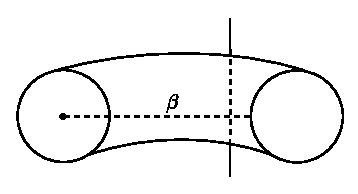
\includegraphics{vol15-figures/fig15-9.eps}}
\end{figure}

\begin{theorem*}
 If $ \sigma_c$ is the abscissa of convergence of $f$ as a
 Dirichlet's series, then $f$ cannot be analytically continued into
 the domain generated by circular discs $\Omega_\zeta$ of radius $\pi
 \bar{D}^. + \varepsilon, \varepsilon > 0$ whose centers $\zeta$ belong
 to a continuum $\mathscr{C}$ which has at least one point $\zeta$
 with $Re \zeta > \sigma$ and at least one point $\zeta'
 \in \mathscr{C}$ with $Re \zeta ' < \sigma_c - B (\bar{D}^., h)$. 
\end{theorem*}

Now, if we continue $f$ with $\zeta$ running along a closed path, we
come back to the original function (see fig.), according to theorem
\ref{chap9:sec2:thm2}, lecture \ref{chap9}, \S \ref{chap9:sec2}. 

\begin{figure}[H]
\centerline{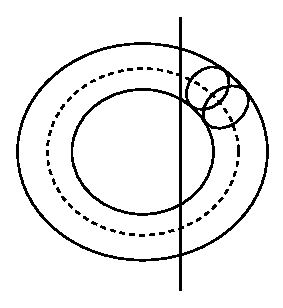
\includegraphics{vol15-figures/fig15-10.eps}}
\end{figure}

It is natural to ask: Is it possible to have such a figure with
singularities inside? In other words, can we have continuation of $f
(Z)$ along a chain of translates $\Omega_\zeta$ whose union forms an
annular region with singularities of $f (Z)$ in the interior of the
bounding curves? We\pageoriginale shall consider this question in a later
lecture. (Lect. \ref{chap16}) 

By the same argument as in $I$, we get a result about the order of
magnitude of $f$ in the plane the whole plane and in a strip. Here
$\mathscr{Y}$ is a horizontal strip, of width $2 \pi \bar{D}^. +
\varepsilon$. 
\begin{theorem*}
 $M (x) \ge K M_\mathscr{Y} (X - B - \varepsilon')$, $K$ depending
 only on $\Lambda, \varepsilon$ and $\varepsilon ( \varepsilon > 0
 , \varepsilon' > 0)$ width $\mathscr{Y} = 2 \pi \bar{D}^. +
 \varepsilon)$ 
\end{theorem*}

Analogous result hold for curvilinear strips.
